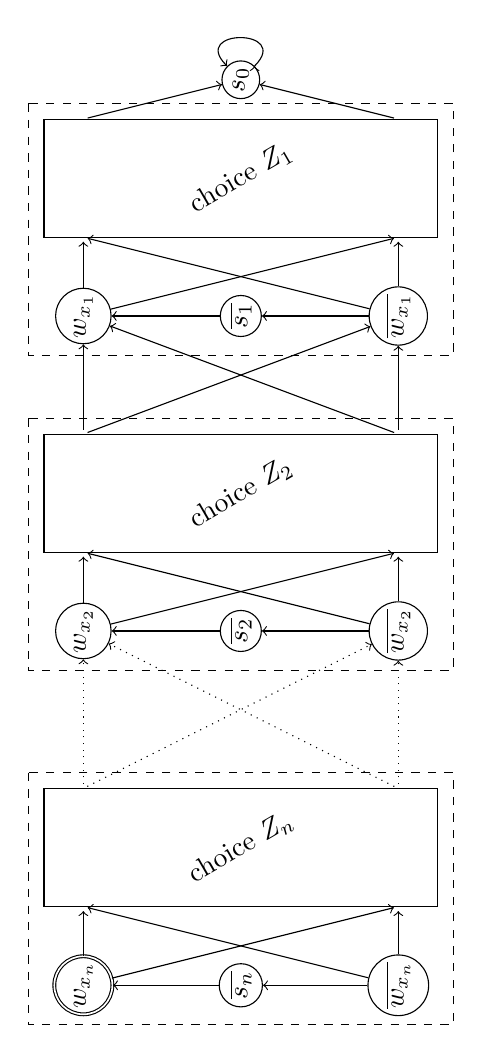
\begin{tikzpicture}[every node/.style={circle, draw, inner sep=1pt}]

\node [rotate=90] (v3) at (-2,0.5) {$w_{x_1}$};
\node [rotate=90] (v2) at (0,0.5) {$\overline{s_1}$};
\node [rotate=90] (v1) at (2,0.5) {$\overline{w_{x_1}}$};
\draw [->] (v1) edge (v2);
\draw [->] (v2) edge (v3);
\draw  (-2.5,3) rectangle (2.5,1.5) node[midway,draw=none,rotate=30] {choice $Z_1$};;

\node [draw=none] (v4) at (-2,1.5) {};
\node [draw=none] (v6) at (2,1.5) {};

\draw [->] (v3) edge (v4);
\draw [->] (v1) edge (v6);


%%%%%
\node [double,rotate=90]  (v13) at (-2,-8) {$w_{x_n}$};
\node [rotate=90] (v12) at (0,-8) {$\overline{s_n}$};
\node [rotate=90] (v11) at (2,-8) {$\overline{w_{x_n}}$};
\draw [->] (v11) edge (v12);
\draw [->] (v12) edge (v13);
\draw  (-2.5,-5.5) rectangle (2.5,-7) node[midway,draw=none,rotate=30] {choice $Z_n$};;

\node [draw=none] (v14) at (-2,-7) {};
\node [draw=none] (v16) at (2,-7) {};

\draw [->] (v13) edge (v14);
\draw [->] (v11) edge (v16);



%%%%
\node [rotate=90] (v23) at (-2,-3.5) {$w_{x_2}$};
\node [rotate=90] (v22) at (0,-3.5) {$\overline{s_2}$};
\node [rotate=90] (v21) at (2,-3.5) {$\overline{w_{x_2}}$};
\draw [->] (v21) edge (v22);
\draw [->] (v22) edge (v23);
\draw  (-2.5,-1) rectangle (2.5,-2.5) node[midway,draw=none,rotate=30] {choice $Z_2$};;

\node [draw=none] (v24) at (-2,-2.5) {};
\node [draw=none] (v26) at (2,-2.5) {};

\draw [->] (v23) edge (v24);
\draw [->] (v21) edge (v26);





\node [draw=none] (v8) at (-2,-5.5) {};
\node [draw=none] (v18) at (2,-5.5) {};
\node [draw=none] (v29) at (2,-1) {};
\node [draw=none] (v19) at (-2,-1) {};
\draw [->, dotted] (v8) edge (v23);
\draw [->, dotted] (v18) edge (v21);
\draw [->] (v19) edge (v3);
\draw [->] (v29) edge (v1);

\node [rotate=90] (v9) at (0,3.5) {$s_0$};
\node [draw=none] (v30) at (-2,3) {};
\draw [->,looseness=5] (v9.south east) edge (v9.north east);

\node [draw=none] (v10) at (2,3) {};

\draw [->] (v19) edge (v1);
\draw [->] (v29) edge (v3);
\draw [->,dotted] (v18) edge (v23);
\draw [->,dotted] (v8) edge (v21);
\draw [->] (v30) edge (v9);
\draw [->] (v10) edge (v9);
\draw [->] (v13) edge (v16);
\draw [->] (v11) edge (v14);
\draw [->] (v23) edge (v26);
\draw [->] (v21) edge (v24);
\draw [->] (v3) edge (v6);
\draw [->] (v1) edge (v4);

\draw [dashed] (-2.7,3.2) rectangle (2.7,0);
\draw [dashed] (-2.7,-0.8) rectangle (2.7,-4);
\draw [dashed] (-2.7,-5.3) rectangle (2.7,-8.5);

%%%%%%%%%
%\node [double] (v33) at (-2,-9) {$y$};
%\draw [->] (v33) edge (v13);
\end{tikzpicture}